\begin{tikzpicture}
	\begin{axis}[
	footnotesize,
	width=\textwidth,
	height=0.8\textheight,
	xticklabels={,,},
	yticklabels={,,},
	ymin=0,
    	ymax=1.5,
	xlabel=solutions,
	ylabel=Gibbs measures
	]
	% \only<1>{\addplot[
	%    red,
	%    domain=-2:2,
	%    samples=201,
	% ]
	%    {exp(-(x+0.25)^2 / (2*0.1)) / (sqrt(0.1 * 2*pi))};
	% \addplot[
	%    blue,
	%    domain=-2:2,
	%    samples=201,
	% ]
	%    {exp(-(x-0.25)^2 / (2*0.1)) / (sqrt(0.1 *2*pi))};
	%    \draw[densely dashed] ({axis cs:-0.25,0}|-{rel axis cs:0,0}) -- ({axis cs:-0.25,0}|-{rel axis cs:0,1});
	%    \draw[densely dashed] ({axis cs:0.25,0}|-{rel axis cs:0,0}) -- ({axis cs:0.25,0}|-{rel axis cs:0,1});}%
	% %%
	% \only<2>{\addplot[
	%    red,
	%    domain=-2:2,
	%    samples=201,
	% ]
	%    {exp(-(x+0.5)^2 / (2*0.1)) / (sqrt(0.1 * 2*pi))};
	% \addplot[
	%    blue,
	%    domain=-2:2,
	%    samples=201,
	% ]
	%    {exp(-(x-0.5)^2 / (2*0.1)) / (sqrt(0.1 *2*pi))};
	%    \draw[densely dashed] ({axis cs:-0.5,0}|-{rel axis cs:0,0}) -- ({axis cs:-0.5,0}|-{rel axis cs:0,1});
	%    \draw[densely dashed] ({axis cs:0.5,0}|-{rel axis cs:0,0}) -- ({axis cs:0.5,0}|-{rel axis cs:0,1});}%
	% %%
	% \only<3>{\addplot[
	%    red,
	%    domain=-2:2,
	%    samples=201,
	% ]
	%    {exp(-(x+1)^2 / (2*0.1)) / (sqrt(0.1 * 2*pi))};
	% \addplot[
	%    blue,
	%    domain=-2:2,
	%    samples=201,
	% ]
	%    {exp(-(x-1)^2 / (2*0.1)) / (sqrt(0.1 *2*pi))};}%
	% \only<3->{%
	% \draw[densely dashed] ({axis cs:-1,0}|-{rel axis cs:0,0}) -- ({axis cs:-1,0}|-{rel axis cs:0,1});
	% \draw[densely dashed] ({axis cs:1,0}|-{rel axis cs:0,0}) -- ({axis cs:1,0}|-{rel axis cs:0,1});}%
	%   %%
	\addplot[
	   red,
	   domain=-2:2,
	   samples=201,
	]
	   {exp(-(x+1)^2 / (2 * 0.5)) / (sqrt(0.3 * 2 * pi))};
	\addplot[
	   blue,
	   domain=-2:2,
	   samples=201,
	]
	   {exp(-(x-1)^2 / (2 * 0.5)) / (sqrt(0.3 * 2 * pi))};%
	% %%
	% \only<5->{\addplot[
	%    red,
	%    domain=-2:2,
	%    samples=201,
	% ]
	%    {exp(-(x+1)^2 / (2* 2)) / (sqrt(2 * 2 * pi))};
	% \addplot[
	%    blue,
	%    domain=-2:2,
	%    samples=201,
	% ]
	%    {exp(-(x-1)^2 / (2* 2)) / (sqrt(2 * 2 * pi))};}
	\end{axis}
	\end{tikzpicture}%